\documentclass[12pt]{article}

% ---------- Packages ----------
\usepackage[margin=1in]{geometry}
\usepackage{amsmath, amssymb}
\usepackage{graphicx}
\usepackage{booktabs}
\usepackage{caption}
\usepackage{setspace}
\usepackage{authblk}
\usepackage[round]{natbib}
\usepackage[hidelinks]{hyperref}
\usepackage{float}

\onehalfspacing
\captionsetup{font=small}

\title{Smoke and Strife: Fire Exposure and Social Conflict in Indonesia}
\author{Hariaksha Gunda\thanks{Email: \href{mailto:hgunda@crimson.ua.edu}{hgunda@crimson.ua.edu}. Code is available at \url{https://github.com/Hariaksha/smoke-and-strife}. This is a shortened version of a longer working paper, which reports the full set of robustness checks. All errors are my own.}}
\affil{The University of Alabama}
\date{Writing sample, \today}

\begin{document}

\maketitle

\begin{abstract}
\noindent Seasonal land and forest fires blanket much of Indonesia in severe air pollution (``haze'') each year. I ask whether exposure to this fire-driven pollution affects social conflict, using fire activity upwind of each of 481 districts, whose smoke the prevailing wind would carry toward the district, as a source of variation driven by wind rather than by local conditions. In districts where conflict is common, more upwind fire reduces monthly conflict events. In proportional terms the effect is similar in all districts, but it is detectable in event counts only where conflict is frequent. The result is robust to excluding the district's own fires, controlling for local weather, and adding next month's fire as a placebo. Two tests point to two channels. Protests fall with smoke from fires in other provinces, which cannot draw on local security forces, consistent with a direct effect of smoke. Events carried out by security forces fall about five times as much as protests in proportional terms, and significantly only with fires in the district's own province, whose fire response the same forces staff, consistent with diversion of state capacity. Fatal events fall more than other events, which argues against a reporting explanation. The negative effect contrasts with evidence that pollution raises individual crime, and suggests that environmental shocks can reduce collective contention both through smoke and by diverting security forces to disaster response.

\medskip
\noindent\textbf{JEL codes:} Q53, Q54, D74, H56 \quad \textbf{Keywords:} air pollution, wildfire, conflict, Indonesia, state capacity
\end{abstract}

\section{Introduction}

A large literature links climate variation to conflict, typically through slow-moving channels such as agricultural income shocks and resource scarcity \citep{hsiang2013quantifying, burkehsiangmiguel2015}. Indonesia offers a different kind of environmental shock. Each dry season, peat and forest fires set to clear land, and intensified by El Ni\~{n}o, produce haze that degrades air quality across much of the western archipelago. Haze is acute, salient, and geographically uneven: it affects outdoor mobility, schools and markets, public health, and the work of the police and military units that respond to fires. Its effect on conflict is not obvious in advance. Studies of air pollution and crime find that pollution raises aggressive and violent behavior \citep{herrnstadt2021, burkhardt2019}, which predicts more conflict. But haze may also keep people indoors and draw security forces into firefighting, which predicts less of the collective and state-led contention recorded in conflict data.

This paper estimates the effect of exposure to fire-driven haze on social conflict at the district-month level. Local fires are a poor measure of exposure, because the land disputes, weak governance, and economic distress that drive conflict may also drive land-clearing fires. I therefore exploit the physics of smoke transport. For each district and month, I measure the total fire radiative power (FRP) of fires that lie \emph{upwind} of the district: within 300\,km and within $45^{\circ}$ of the direction the wind blows from. Conditional on district and year-month fixed effects, this upwind fire activity changes the district's smoke exposure through the wind but is plausibly unrelated to the district's own political and economic shocks. I build the measure for 481 districts (\emph{kabupaten} and \emph{kota}), linking NASA VIIRS fire detections, ERA5 wind fields, and ACLED conflict events in a panel of 60,125 district-months from 2015 to 2025.

The main evidence is the reduced form: the effect of upwind fire on conflict, which requires only that wind-driven variation in upwind fire is unrelated to local conflict shocks. In districts where conflict occurs in at least 30\% of months, a one-log-point increase in upwind FRP reduces conflict events by 0.026 per district-month ($p=0.002$), about 1.9\% of the mean. Across all districts the estimate is small and insignificant. These results are consistent: when districts are grouped by their conflict history \emph{before} the estimation window, the effect in levels grows steadily with prior conflict, but in proportional terms it is about the same everywhere. Upwind fire appears to reduce conflict by a small, similar percentage in all districts, which is measurable only where conflict is frequent. In September and October 2015, at the height of that year's haze, upwind fire in these districts was 1.5 to 2.3 log points above its usual level for those months, which the estimate translates into about 3--4\% fewer conflict events.

The result survives the main threats to identification. Next month's upwind fire does not predict this month's conflict. The estimate is unchanged when fires inside the district are excluded from the upwind measure, and when local rainfall and temperature, which drive both fire and agricultural income, are controlled for. It is larger in 2018--2025, when ACLED's coverage of Indonesia is more complete, and it is smaller but still significant when Papua, the site of an active insurgency, is excluded. A placebo instrument built from fires upwind of a distant district has no effect.

I then ask why conflict falls. If haze kept people indoors, protests should fall most. If it diverted police and military units to fire response, events carried out by state forces should fall most. If it crowded out conflict reporting, low-salience and imprecisely recorded events should fall most. In proportional terms, events carried out by state forces fall by about 6\% per log point of upwind fire, about five times as much as peaceful protests; fatal events, the least likely to go unreported, fall more than other events; and imprecisely recorded events do not fall. A further test separates smoke from fire response. Indonesia organizes its fire task forces by province, with the provincial military commander and police chief as deputy commanders, so fires in a district's own province draw on its security forces, while fires in another province reach it only as smoke. The decline in protests comes from other-province fire, which points to a direct effect of smoke. The decline in state violence is significant only for same-province fire, consistent with the diversion of security forces, although the other-province estimate is too imprecise to reject equal effects.

The paper contributes to three literatures. First, it adds to work on pollution and behavior \citep{herrnstadt2021, bondyrothsager2020, burkhardt2019}, which finds that short-run pollution increases individual crime. I find the opposite sign for collective and state-led contention. Second, it adds to the climate-and-conflict literature by documenting acute channels that operate within the month, through smoke itself and through the state's response to environmental disasters. Third, it brings district-level evidence to the political-science debate over whether disasters raise or lower conflict and repression \citep{nelrigharts2008, slettebak2012, woodwright2016}, by isolating a recurring disaster whose response demonstrably draws on the security forces.

\section{Setting and Related Literature}
\label{sec:lit}

\paragraph{Indonesian haze.} Indonesian fires are mostly set to clear land for plantations and agriculture, and in El Ni\~{n}o years they burn out of control in drained peatlands. The resulting haze is a severe pollution shock: smoke from the 1997 fires caused an estimated 15,600 fetal, infant, and child deaths \citep{jayachandran2009}, and fire emissions in strong El Ni\~{n}o years raise regional adult cardiovascular mortality by about 2\% \citep{marlier2013}. \citet{sheldonsankaran2017} use Indonesian FRP to instrument Singaporean air pollution, but aggregate fires across all of Indonesia because they lack consistent wind data. The upwind measure here adds that directional refinement at the district level.

\paragraph{Pollution and behavior.} Wind-based designs show that pollution raises crime. \citet{herrnstadt2021} find that violent crime rises by 1.9\% on the downwind side of Chicago interstates; \citet{bondyrothsager2020} find that a 10-point increase in London's air quality index raises crime by 2.6\%; and \citet{burkhardt2019} find that PM2.5 raises violent crime across US counties. These studies concern individual acts. The events in conflict data are collective or organized, and may respond differently.

\paragraph{Disasters, state capacity, and conflict.} Political scientists disagree on how disasters affect conflict. \citet{nelrigharts2008} find that disasters raise the risk of civil conflict, in part because they weaken state capacity, while \citet{slettebak2012} finds that climate-related disasters lower it. \citet{woodwright2016} find that governments escalate repression after rapid-onset disasters. Evidence from economics shows that the deployment of security forces has measurable effects: redeploying police in London after the 2005 terror attacks reduced crime where they were sent \citep{dracamachinwitt2011}. The closest Indonesian precedent is \citet{lu2023fish}, who use a spatial design to show that fish catches raise conflict, with protests and riots the most responsive event types.

\paragraph{Fire response and the security forces.} Presidential instructions issued during the 2015 fires and again in 2020 direct the armed forces (TNI) and national police (Polri) to deploy personnel to extinguish land and forest fires and to patrol fire-prone areas \citep{inpres11_2015, inpres3_2020}. Under the 2020 instruction, governors and district heads command provincial and district fire task forces, with the provincial or district military commander and police chief as deputy commanders. Fire emergencies therefore draw on the personnel and leadership of the same security forces whose actions conflict data record, and they do so province by province.

\section{Data}
\label{sec:data}

\paragraph{Fires.} Fire detections come from the NASA VIIRS active fire product (375\,m, Suomi-NPP). I keep vegetation fires with high or nominal confidence. Each detection has a location, date, and fire radiative power (FRP, in megawatts), which measures fire intensity.

\paragraph{Wind.} Monthly 10\,m wind components come from ERA5 reanalysis \citep{hersbach2023era5} on a $0.25^{\circ}$ grid. A district's monthly wind direction is the direction implied by the average wind components over the grid cells it contains, or the nearest cell for small districts. Monthly precipitation and temperature from ERA5 are aggregated in the same way and used as controls.

\paragraph{Conflict.} Conflict events come from the Armed Conflict Location \& Event Data Project (ACLED), from January 2015 to June 2025. I assign each event to the GADM Level-2 district polygon that contains its coordinates rather than using ACLED's district names, which merge cities with the surrounding regencies; all 21,653 events in the sample window are assigned. The main outcome is the monthly count of all events. I also study political violence (riots, violence against civilians, battles, and explosions) and, for the mechanism tests, finer counts by event type, actor, source, and precision.

\paragraph{Panel.} The panel covers the 481 districts that record at least one event, observed in each of 125 months (February 2015 to June 2025), for 60,125 district-months. Conflict is rare: 82.9\% of district-months record no event, and the mean is 0.36 events. Conflict is concentrated in Java, Sumatra, and Papua, while fires are concentrated in Sumatra, Kalimantan, and Papua, so many conflict-prone districts lie near major fire regions without burning heavily themselves.

\section{Empirical Strategy}
\label{sec:empirical}

\paragraph{The upwind measure.} For district $d$ in month $t$, upwind fire activity is
\[
Z_{dt} = \sum_{f \in \mathcal{U}_{dt}} \text{FRP}_f,
\]
where $\mathcal{U}_{dt}$ contains the fire detections in month $t$ that lie within 300\,km of the district's centroid and within $\pm 45^{\circ}$ of the direction its wind blows from. These are fires whose smoke the wind would carry toward the district. It enters regressions as $\text{logZ}_{dt} = \log(1+Z_{dt})$.

\paragraph{Reduced form.} The main specification is
\begin{equation}
y_{dt} = \alpha_d + \gamma_t + \pi_0\, \text{logZ}_{dt} + \pi_1\, \text{logZ}_{d,t-1} + \varepsilon_{dt},
\label{eq:rf}
\end{equation}
where $y_{dt}$ is a conflict count, $\alpha_d$ are district fixed effects, and $\gamma_t$ are year-month fixed effects, which absorb national shocks and seasonality. The lag allows smoke and its consequences to persist into the next month. Standard errors are clustered by province (34 clusters). The coefficient of interest, $\pi_0$, is the effect of wind-borne exposure to upwind fire on conflict. It is identified if, after removing district and year-month means, the month-to-month variation in upwind fire created by the wind is unrelated to the district's own conflict shocks. Because the wind direction that defines ``upwind'' changes from month to month, the measure picks up different fires in different months for the same district.

\paragraph{Threats to identification.} Three threats are most important. First, regional seasonality or regional shocks such as droughts could raise both upwind fire and local conflict; I test this with leads of the instrument, weather controls, and province-by-calendar-month fixed effects. Second, the upwind cone begins at the district centroid, so it includes some fires inside the district, which could have local causes; I rebuild the measure without them. Third, reporting of conflict could itself respond to haze; Section~\ref{sec:mechanisms} tests the predictions of a reporting explanation.

\paragraph{Why not instrument local fire?} Upwind fire strongly predicts a district's own fire intensity (effective $F = 81.3$; \citealp{montielolea2013}), so it could serve as an instrument for local fire. But that IV would require upwind fire to affect conflict only through local fire, which fails if smoke changes behavior, the very mechanism of interest. I therefore treat the reduced form as the main evidence. Section~\ref{sec:pollution} reports an IV in which upwind fire instruments a direct measure of pollution, an exclusion restriction consistent with the proposed mechanism.

\section{Results}
\label{sec:results}

\subsection{Upwind fire and conflict}

Table~\ref{tab:rf} reports the reduced form for four outcomes, in the full panel and in the 85 ``conflict-active'' districts that record conflict in at least 30\% of months. In the full panel, all four coefficients are negative but small and insignificant. In the conflict-active districts, a one-log-point increase in upwind FRP reduces all events by 0.026 per district-month ($p=0.002$), 1.9\% of the mean, and the Anderson--Rubin test, which is robust to weak instruments, rejects a zero effect ($p=0.012$). The decline in political violence is smaller in absolute terms and less precisely estimated ($p=0.078$). Within political violence, it comes from riots and violence against civilians.

\begin{table}[!htbp]
\centering
\caption{Reduced form: effect of upwind fire on monthly conflict events}
\label{tab:rf}
\small
\begin{tabular}{lcccc}
\toprule
 & All events & Political violence & Riots and VAC & VAC \\
\midrule
\multicolumn{5}{l}{\emph{Full panel (481 districts, 60,125 district-months)}} \\
$\text{logZ}_{dt}$ & $-0.0024$ & $-0.0008$ & $-0.0008$ & $-0.0007$ \\
 & (0.0020) & (0.0006) & (0.0006) & (0.0005) \\
Mean of outcome & 0.360 & 0.059 & & \\
\addlinespace
\multicolumn{5}{l}{\emph{Conflict-active districts (85 districts, 10,625 district-months)}} \\
$\text{logZ}_{dt}$ & $-0.0261^{***}$ & $-0.0072^{*}$ & $-0.0079^{**}$ & $-0.0055^{*}$ \\
 & (0.0078) & (0.0039) & (0.0037) & (0.0029) \\
Mean of outcome & 1.398 & 0.220 & 0.167 & 0.072 \\
Anderson--Rubin $p$ & 0.012 & 0.164 & 0.066 & 0.024 \\
\bottomrule
\end{tabular}
\begin{minipage}{0.95\textwidth}
\vspace{4pt}
\footnotesize \emph{Notes:} Coefficient on contemporaneous log upwind FRP from Eq.~\eqref{eq:rf}, which also includes its one-month lag and district and year-month fixed effects. Standard errors clustered by province (34 clusters) in parentheses. VAC is violence against civilians. Conflict-active districts record at least one event in at least 30\% of months. The Anderson--Rubin test is the joint test that both instrument coefficients are zero, for the IV of local fire on the outcome. $^{***}p<0.01$, $^{**}p<0.05$, $^{*}p<0.1$.
\end{minipage}
\end{table}

\subsection{Is the conflict-active cutoff driving the result?}
\label{sec:propensity}

The 30\% cutoff was not chosen in advance and is measured over the same months used for estimation. To avoid both problems, I measure each district's conflict history before the estimation window, as the number of months in 2015--2017 with any ACLED event, and estimate the reduced form on 2018--2025 separately for districts with 0, 1, 2--5, and 6 or more such months. As a second measure that keeps the full sample, I compute each district-year's conflict propensity from all \emph{other} years and group districts into quintiles.

\begin{figure}[!htbp]
\centering
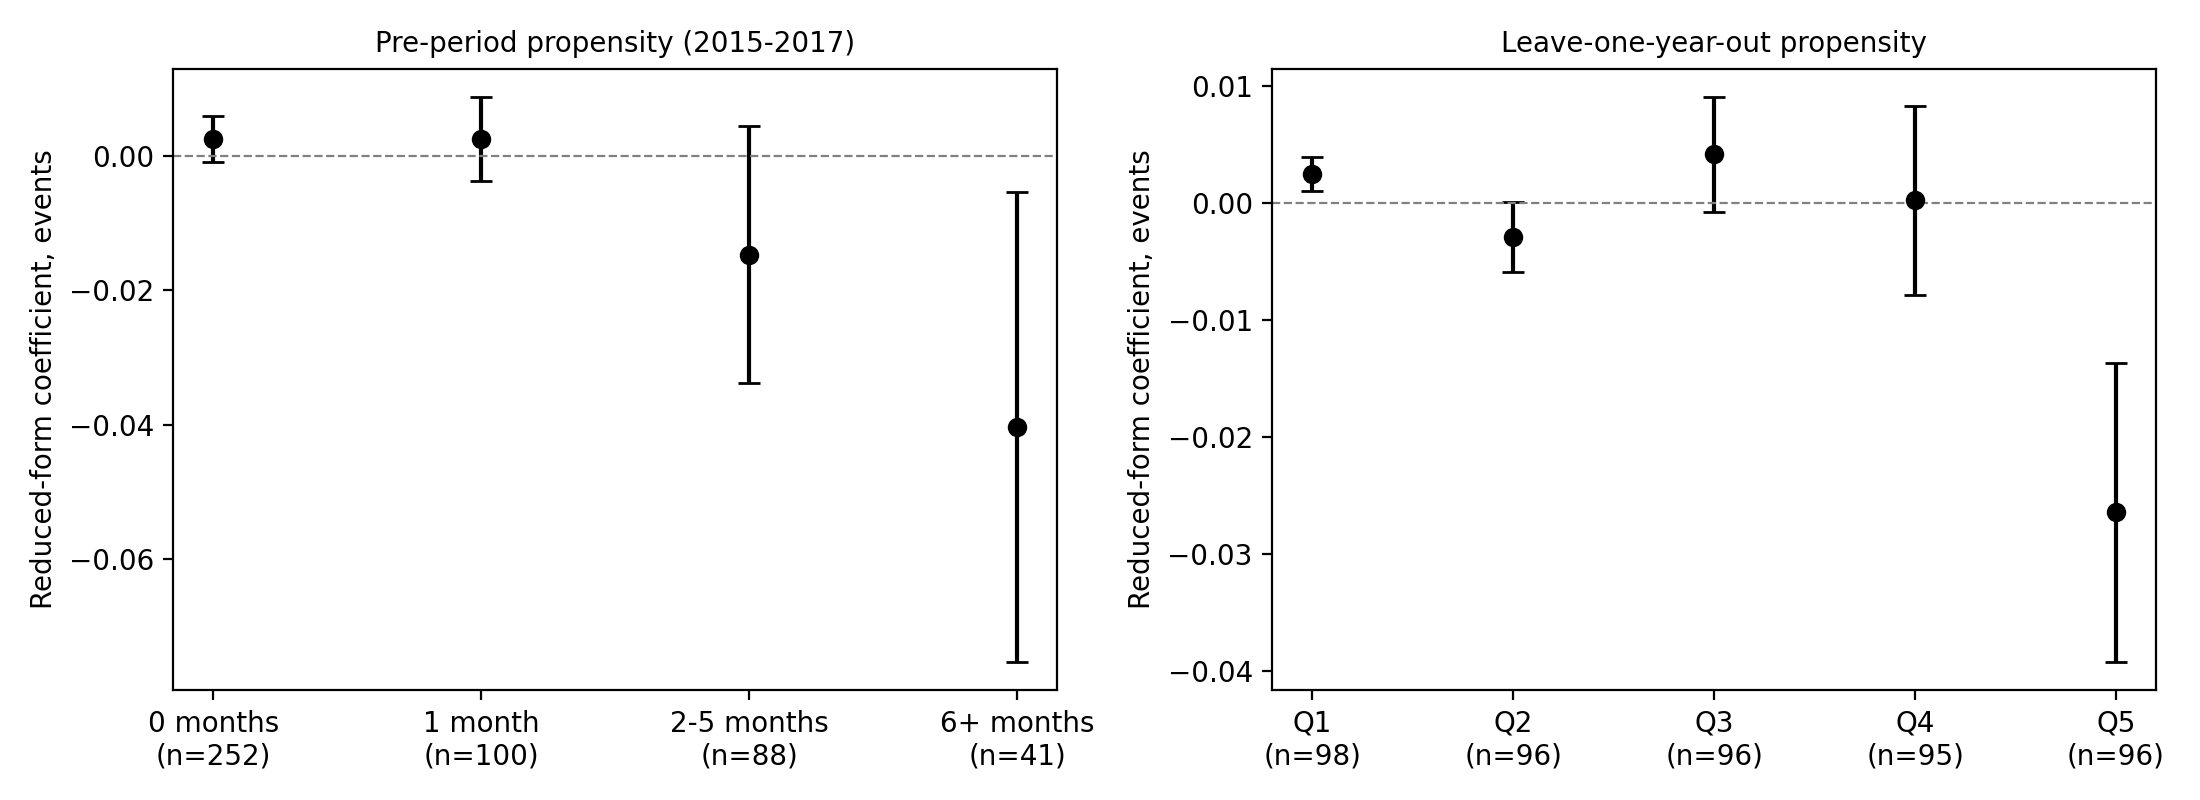
\includegraphics[width=\textwidth]{figures/conflict_propensity_bins.png}
\caption{Reduced-form effect of upwind fire by prior conflict propensity. Each point is the coefficient on contemporaneous log upwind FRP, estimated separately for each group, with 95\% confidence intervals from province-clustered standard errors. Left: districts grouped by months with any event in 2015--2017, estimated on 2018--2025. Right: quintiles of leave-one-year-out conflict propensity, estimated on 2015--2025.}
\label{fig:propensity}
\end{figure}

Figure~\ref{fig:propensity} shows a gradient rather than a threshold. The effect is close to zero in districts with no or one month of prior conflict ($+0.003$), turns negative for two to five months ($-0.015$, $p=0.14$), and is largest for the 41 districts with six or more ($-0.040$, $p=0.037$). The leave-one-year-out quintiles give the same picture. A Poisson version of the same regression, which estimates proportional effects, finds no gradient: the effect is about $-1\%$ per log point regardless of prior conflict (interaction $p=0.60$). Upwind fire therefore appears to reduce conflict by a similar small percentage everywhere, which is detectable in event counts only where conflict is common. This explains the full-sample null without a mechanism specific to conflict-prone districts.

\subsection{Robustness}
\label{sec:robustness}

Table~\ref{tab:robust} reports the all-events reduced form in the conflict-active districts under the main robustness checks.

\begin{table}[!htbp]
\centering
\caption{Robustness of the reduced form, all events, conflict-active districts}
\label{tab:robust}
\small
\begin{tabular}{lccc}
\toprule
Specification & Districts & Coefficient on $\text{logZ}_{dt}$ & $p$-value \\
\midrule
Baseline & 85 & $-0.0261$ & 0.002 \\
\addlinespace
\multicolumn{4}{l}{\emph{Regional seasonality and weather}} \\
\quad + one-month lead of the instrument & 85 & $-0.0256$ & 0.001 \\
\quad\quad lead coefficient & & $-0.0002$ & 0.985 \\
\quad + precipitation and temperature (and lags) & 85 & $-0.0262$ & 0.002 \\
\quad + weather and province $\times$ calendar-month FE & 85 & $-0.0262$ & 0.013 \\
\quad + province $\times$ year-month FE & 85 & $-0.0277$ & 0.190 \\
\addlinespace
\multicolumn{4}{l}{\emph{Measurement and sample}} \\
\quad Instrument excludes fires inside the district & 85 & $-0.0294$ & 0.004 \\
\quad 2018--2025 only & 85 & $-0.0362$ & 0.003 \\
\quad 2018--2025, districts re-selected on 2018--2025 & 117 & $-0.0303$ & 0.002 \\
\quad Excluding Papua and Papua Barat & 70 & $-0.0200$ & 0.041 \\
\addlinespace
\multicolumn{4}{l}{\emph{Placebo}} \\
\quad Upwind fire of a random district $\geq 500$\,km away & 85 & $+0.0023$ & 0.802 \\
\bottomrule
\end{tabular}
\begin{minipage}{0.95\textwidth}
\vspace{4pt}
\footnotesize \emph{Notes:} Each row reports the coefficient on contemporaneous log upwind FRP in Eq.~\eqref{eq:rf} with all events as the outcome, modified as indicated; the ``lead coefficient'' row reports the coefficient on next month's upwind FRP, and the placebo row the coefficient on the distant district's upwind FRP. District and year-month fixed effects in all rows; standard errors clustered by province.
\end{minipage}
\end{table}

\paragraph{Regional shocks.} If upwind fire captured regional seasonal trends, next month's upwind fire would also predict this month's conflict. It does not (lead coefficient $-0.0002$, $p=0.985$). Drought raises fire activity and could affect conflict through income, but controlling for district precipitation and temperature leaves the estimate unchanged, although upwind fire is clearly related to rainfall (correlation $-0.36$). Adding province-by-calendar-month fixed effects, which absorb each province's seasonal fire cycle, on top of the weather controls also leaves it unchanged. Province-by-year-month fixed effects, which absorb any shock common to a province in a given month, leave the point estimate almost identical but remove most of the variation, so it is no longer significant. This check cannot rule out province-wide shocks, but the stable point estimate is reassuring.

\paragraph{Own fires, coverage, and Papua.} Fires inside the district account for 4.9\% of upwind FRP; excluding them leaves the estimate unchanged, so the result does not come from local burning. ACLED's coverage of Indonesia roughly triples in 2018, and restricting to 2018--2025 strengthens the result. Papua contains 15 of the 85 conflict-active districts and an active separatist insurgency, and accounts for 62\% of events carried out by state forces. Excluding it shrinks the estimate to $-0.020$ ($p=0.041$; Anderson--Rubin $p=0.081$), so Papua contributes to the headline result, but the mechanism results below hold without it.

\paragraph{Inference.} The all-events result remains significant at the 5\% level when the IV of local fire is estimated with Conley standard errors that allow spatial correlation across province boundaries ($p \approx 0.03$), and the reduced form remains significant after a false-discovery-rate correction across the four outcomes in Table~\ref{tab:rf} (sharpened $q=0.009$; \citealp{anderson2008multiple}). The political-violence result is less robust and I treat it as suggestive.

\section{Mechanisms}
\label{sec:mechanisms}

\subsection{Which events decline?}

Three explanations make different predictions about which events decline. \emph{Avoidance}: haze keeps people indoors, so protests and other crowd events should fall most. \emph{State-capacity diversion}: security forces are redeployed to fire response, so events carried out by state forces should fall most. \emph{Reporting}: haze or fire coverage crowds out conflict reporting, so events reported by local sources and events located or dated imprecisely should fall most, and fatal events, which are hard to miss, should fall least. Because the outcomes differ greatly in frequency, Table~\ref{tab:mechanisms} reports Poisson (PPML) estimates of Eq.~\eqref{eq:rf}, whose coefficients are proportional effects and comparable across outcomes.

\begin{table}[!htbp]
\centering
\caption{Proportional effects of upwind fire by event type, actor, and reporting (conflict-active districts)}
\label{tab:mechanisms}
\small
\begin{tabular}{lccc}
\toprule
Outcome (district-month count) & Mean & PPML coef. (SE) & $p$-value \\
\midrule
All events & 1.398 & $-0.013$ (0.006) & 0.030 \\
\addlinespace
\multicolumn{4}{l}{\emph{Event type}} \\
\quad Peaceful protests & 1.077 & $-0.014$ (0.006) & 0.017 \\
\quad Riots & 0.095 & $-0.012$ (0.021) & 0.565 \\
\quad Violence against civilians & 0.072 & $-0.067$ (0.016) & $<0.001$ \\
\quad Battles & 0.044 & $-0.024$ (0.017) & 0.172 \\
\addlinespace
\multicolumn{4}{l}{\emph{Actor}} \\
\quad Carried out by state forces & 0.068 & $-0.063$ (0.017) & $<0.001$ \\
\quad Non-state violence (riots, VAC, battles) & 0.164 & $-0.010$ (0.016) & 0.513 \\
\addlinespace
\multicolumn{4}{l}{\emph{Reporting}} \\
\quad National sources & 1.234 & $-0.011$ (0.006) & 0.096 \\
\quad Local or subnational sources & 0.148 & $-0.025$ (0.020) & 0.210 \\
\quad Imprecisely located or dated & 0.072 & $+0.001$ (0.030) & 0.962 \\
\quad Fatal events & 0.056 & $-0.052$ (0.019) & 0.007 \\
\bottomrule
\end{tabular}
\begin{minipage}{0.95\textwidth}
\vspace{4pt}
\footnotesize \emph{Notes:} Poisson pseudo-maximum-likelihood estimates of Eq.~\eqref{eq:rf}; coefficient on contemporaneous log upwind FRP. ``Carried out by state forces'' means ACLED's primary actor is the police or military. Imprecise events have ACLED geographic or time precision codes above 1. District and year-month fixed effects; standard errors clustered by province.
\end{minipage}
\end{table}

The largest proportional declines are in events carried out by state forces ($-6.3\%$ per log point, $p<0.001$) and in violence against civilians ($-6.7\%$), about five times the decline in peaceful protests ($-1.4\%$, $p=0.017$). Protests account for most of the decline in the \emph{number} of events only because they are by far the most common event type. Non-state violence as a whole does not decline. The reporting explanation fits poorly: events from national sources fall in proportion to all events, imprecisely recorded events do not fall at all, and fatal events, the least likely to go unreported, fall by 5\% per log point, four times as much as all events. Finally, conflict is not merely postponed: adding two further monthly lags of upwind fire, every lag coefficient for all events is negative, and the four-month cumulative effect ($-0.037$, $p=0.030$) is larger than the contemporaneous effect alone.

\subsection{Smoke or fire response?}
\label{sec:province}

The test above leaves a gap. Upwind fire often burns in other districts, so it is not obvious why it should draw on the security forces of the district that receives the smoke. Indonesia's fire-response arrangements suggest a sharper test. Because fire task forces are organized by province, fires in a district's own province draw on its security forces, while fires in another province reach it only as smoke. If the decline in state violence reflects the diversion of security forces, it should respond mainly to same-province fire; if it reflects smoke, the source province should not matter.

I split each upwind fire's FRP into a same-province and an other-province component according to where it burns. Same-province fires account for 54\% of upwind FRP, and the two components are only weakly correlated (0.23), so their effects can be estimated separately. Table~\ref{tab:province} reports the reduced form with both components.

\begin{table}[!htbp]
\centering
\caption{Same-province and other-province upwind fire (conflict-active districts, PPML)}
\label{tab:province}
\small
\begin{tabular}{lccc}
\toprule
 & Same-province & Other-province & Equality \\
Outcome & coef. (SE) & coef. (SE) & $p$-value \\
\midrule
All events & $-0.004$ (0.008) & $-0.013^{**}$ (0.005) & 0.347 \\
Peaceful protests & $-0.003$ (0.007) & $-0.018^{***}$ (0.005) & 0.078 \\
Carried out by state forces & $-0.045^{***}$ (0.017) & $-0.038$ (0.043) & 0.880 \\
Violence against civilians & $-0.064^{***}$ (0.016) & $-0.028$ (0.035) & 0.363 \\
VAC by state forces & $-0.068^{***}$ (0.017) & $-0.048$ (0.047) & 0.702 \\
Non-state violence & $-0.001$ (0.025) & $+0.005$ (0.019) & 0.875 \\
\bottomrule
\end{tabular}
\begin{minipage}{0.95\textwidth}
\vspace{4pt}
\footnotesize \emph{Notes:} Poisson reduced form with log same-province and log other-province upwind FRP and the one-month lag of each; coefficients on the contemporaneous components. ``Equality'' tests that the two coefficients are equal. District and year-month fixed effects; standard errors clustered by province. $^{***}p<0.01$, $^{**}p<0.05$, $^{*}p<0.1$.
\end{minipage}
\end{table}

The two kinds of event respond to different fires. The decline in protests comes from other-province fire ($-1.8\%$ per log point, $p=0.001$), while same-province fire has no detectable effect on protests; the difference is marginally significant ($p=0.078$). Because fires in another province cannot draw on the district's security forces, this decline is best explained by the smoke itself. Events carried out by state forces fall significantly only with same-province fire ($-4.5\%$, $p=0.009$), as does violence against civilians by state forces ($-6.8\%$, $p<0.001$). The other-province estimates are similar in size but imprecise, so I cannot reject equal effects. Outside Papua, both patterns remain: protests still respond to other-province fire ($-1.7\%$, $p=0.002$), and state-force events fall by a larger percentage ($-10.0\%$, $p=0.006$), mainly with same-province fire ($-6.9\%$, $p=0.055$, against $-2.8\%$, $p=0.51$ for other-province fire).

Two caveats apply. Same-province fires are on average closer to the district, so the contrast is partly between near and far fires, and the data are too collinear to separate the two. And during the largest fires, security forces from neighboring provinces may also be deployed, which would blur the contrast. With these caveats, the evidence suggests two channels: smoke reduces protests, and the diversion of security forces to fire response plausibly reduces state violence. The evidence for the first channel is firmer.

\section{Instrumenting Pollution Directly}
\label{sec:pollution}

If smoke is a channel, upwind fire should raise measured pollution, and pollution should reduce conflict. I use monthly surface PM2.5 from the MERRA-2 aerosol reanalysis \citep{gelaro2017merra}, constructed following \citet{buchard2016}, and instrument log PM2.5 with log upwind FRP and its lag. This IV assumes that upwind fire affects conflict only through the pollution it carries, which is the mechanism under study.

Upwind fire strongly predicts PM2.5 (effective $F = 41.1$ in the full panel and 25.7 in conflict-active districts). In conflict-active districts, instrumented PM2.5 reduces conflict events ($-1.23$, Anderson--Rubin $p=0.004$): a 10\% increase in PM2.5 reduces events by about 8\% of the mean. The estimate changes little when the district's own fire intensity is controlled for ($-1.07$, Anderson--Rubin $p=0.023$), so it does not reflect local burning.

Two limitations keep this from being conclusive. MERRA-2 is a model whose fire emissions are derived from satellite fire detections, so part of its first stage may be mechanical. And satellite-observed aerosol optical depth from MODIS MAIAC does not respond detectably to upwind fire (effective $F = 4.2$ in conflict-active districts), plausibly because clouds and thick smoke remove the haziest days from the satellite record. I therefore treat the pollution IV as suggestive of a pollution channel, not as confirmation of it.

\section{Discussion and Conclusion}
\label{sec:conclusion}

Wind-borne exposure to fire reduces conflict in Indonesia. The effect is a small percentage decline that is measurable where conflict is common, and it is robust to excluding local fires, to weather controls, to leads of the instrument, and to restricting to the years with better conflict coverage. The pattern of declines points to two channels. Protests fall with smoke from fires in other provinces, which suggests that smoke itself discourages collective action. Events carried out by security forces fall about five times as much as protests in proportional terms, and mainly with fires in the district's own province, which is consistent with the diversion of security forces to fire response.

The negative sign contrasts with two literatures. Climate shocks usually increase conflict through income and resource scarcity \citep{hsiang2013quantifying, burkehsiangmiguel2015}, and pollution usually increases individual crime \citep{herrnstadt2021, bondyrothsager2020, burkhardt2019}. The difference is plausibly one of horizon and outcome. Haze is an acute shock that operates through logistics, keeping people indoors and keeping security forces busy, rather than a persistent shock to income. And the events in conflict data are collective or organized acts that depend on coordination and on the operational capacity of the security forces, unlike the individual acts studied in the pollution-crime literature. Pollution could raise individual irritability while reducing organized contention.

Several limitations remain. The effect is measured where conflict is frequent and is weaker without Papua. Province-wide shocks cannot be ruled out, because province-by-year-month fixed effects leave too little variation. The state-capacity channel is inferred from the composition of conflict events rather than from observed deployments, and the pollution channel is not yet confirmed with observed pollution. Records of police and military participation in fire response, daily matching of satellite or ground-monitor pollution to conflict events, and replication in other fire-prone countries such as Brazil would sharpen these conclusions.

\bibliographystyle{plainnat}
\bibliography{references}

\end{document}
